\documentclass[10pt,letterpaper]{article} 
\usepackage{tikz}
\usepackage{tools}
\usepackage{enumitem,caption}
\usepackage{listings}
\lstset{language=Python}
%\lstset{frame=lines}
%\lstset{caption={Insert code directly in your document}}
\lstset{label={lst:code_direct}}
\lstset{basicstyle=\footnotesize}

%\usepackage{graphicx}‎‎
%\usefonttheme{serif}‎
%\usepackage{ptext}‎
%\usepackage{xepersian}
%\settextfont{B Nazanin}
\usepackage{lipsum}
\setlength{\parindent}{0pt}
\newcommand{\pf}{$\blacksquare$}

\newcommand{\Span}{\text{Span}}
\newcommand{\NF}{\text{NF}}
\newcommand{\EDFA}{\text{EDFA}}
\newcommand{\ASE}{\text{ASE}}

\newcommand{\bns}{\textit{broadcast-and-select}  architecture}
\newcommand{\Bns}{\textit{Broadcast-and-select} architecture}

\newcommand{\rns}{\textit{route-and-select} architecture}
\newcommand{\Rns}{\textit{Route-and-select} architecture}

\newcounter{QuestionNumber}
\setcounter{QuestionNumber}{1}

\newcommand{\temp}{{\color{red}{temp}}}

\newcommand{\Q}{
\textbf{Question \theQuestionNumber)}
\stepcounter{QuestionNumber}
}
\newcommand{\EX}{\Bbb E}
\newcommand{\nl}{\newline\newline}
\begin{document}
\large
\begin{center}
In the name of beauty

The 6th problem set solution of Optical Networks course
\hl
\end{center}
\Q
\begin{enumerate}[label=\alph*-]
\item
Any extra regeneration imposes cost to our design due to the expense of electronical devices deployed for them. To this reason, a lower amount of regeneration is more favorable. This argument holds in both all-optical or O-E-O network architectures.
\item
RWA contains wavelength assignment as a subproblem, whereas RSA consists of routing and spectrum assignment. It is said that spectrum allocation provides a finer granularity against wavelength and channel bandwidths can be settled in an elastic manner. The problem of RSA is generally more efficient, though more complicated and costly (if the optical and electrical devices are not designed to perform in elastic networks).
\item
Any signal undergoing an electrical infrastructure experiences 3R regeneration, which is the case here since transponders provide interfaces between two different optical domains (L-band and C-band). Amplifiers, on the other hand, typically provide only a 1R regeneration (that is, they only re-amplify the signal).
\item
An example is as follows:
\begin{figure}[h]
\centering
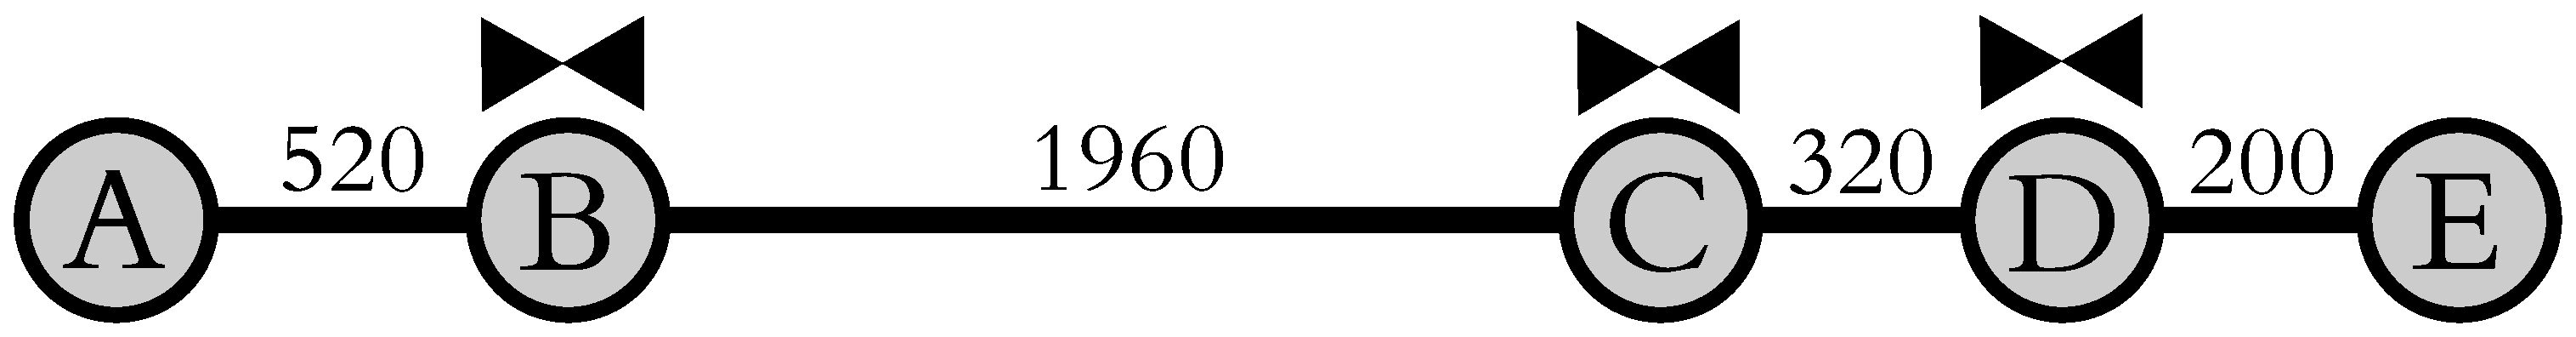
\includegraphics[width=90mm]{regeneration}
\end{figure}
where regeneration takes place at nodes B and C for optical reach considerations and at node D since a same free wavelength cannot be found on links CD and DE. The potential need for extra regeneration comes from our constraints in regenerating signal only at nodes. To this reason, a length profile containing diverse link lengths may give rise to such scenarios with extra regeneration.
\end{enumerate}
\Q

\begin{enumerate}[label=\alph*-]
\item
The steps of the Bhandari's algorithm are as indicated in figure \ref{fig:bhandari}.
\item
The steps of the Suurballe's algorithm are as indicated in figure \ref{fig:suurballe}.
\end{enumerate}

\begin{figure}[h]
\centering
%%%%%%%%%%%%%%%%%
\begin{subfigure}{0.49\textwidth}
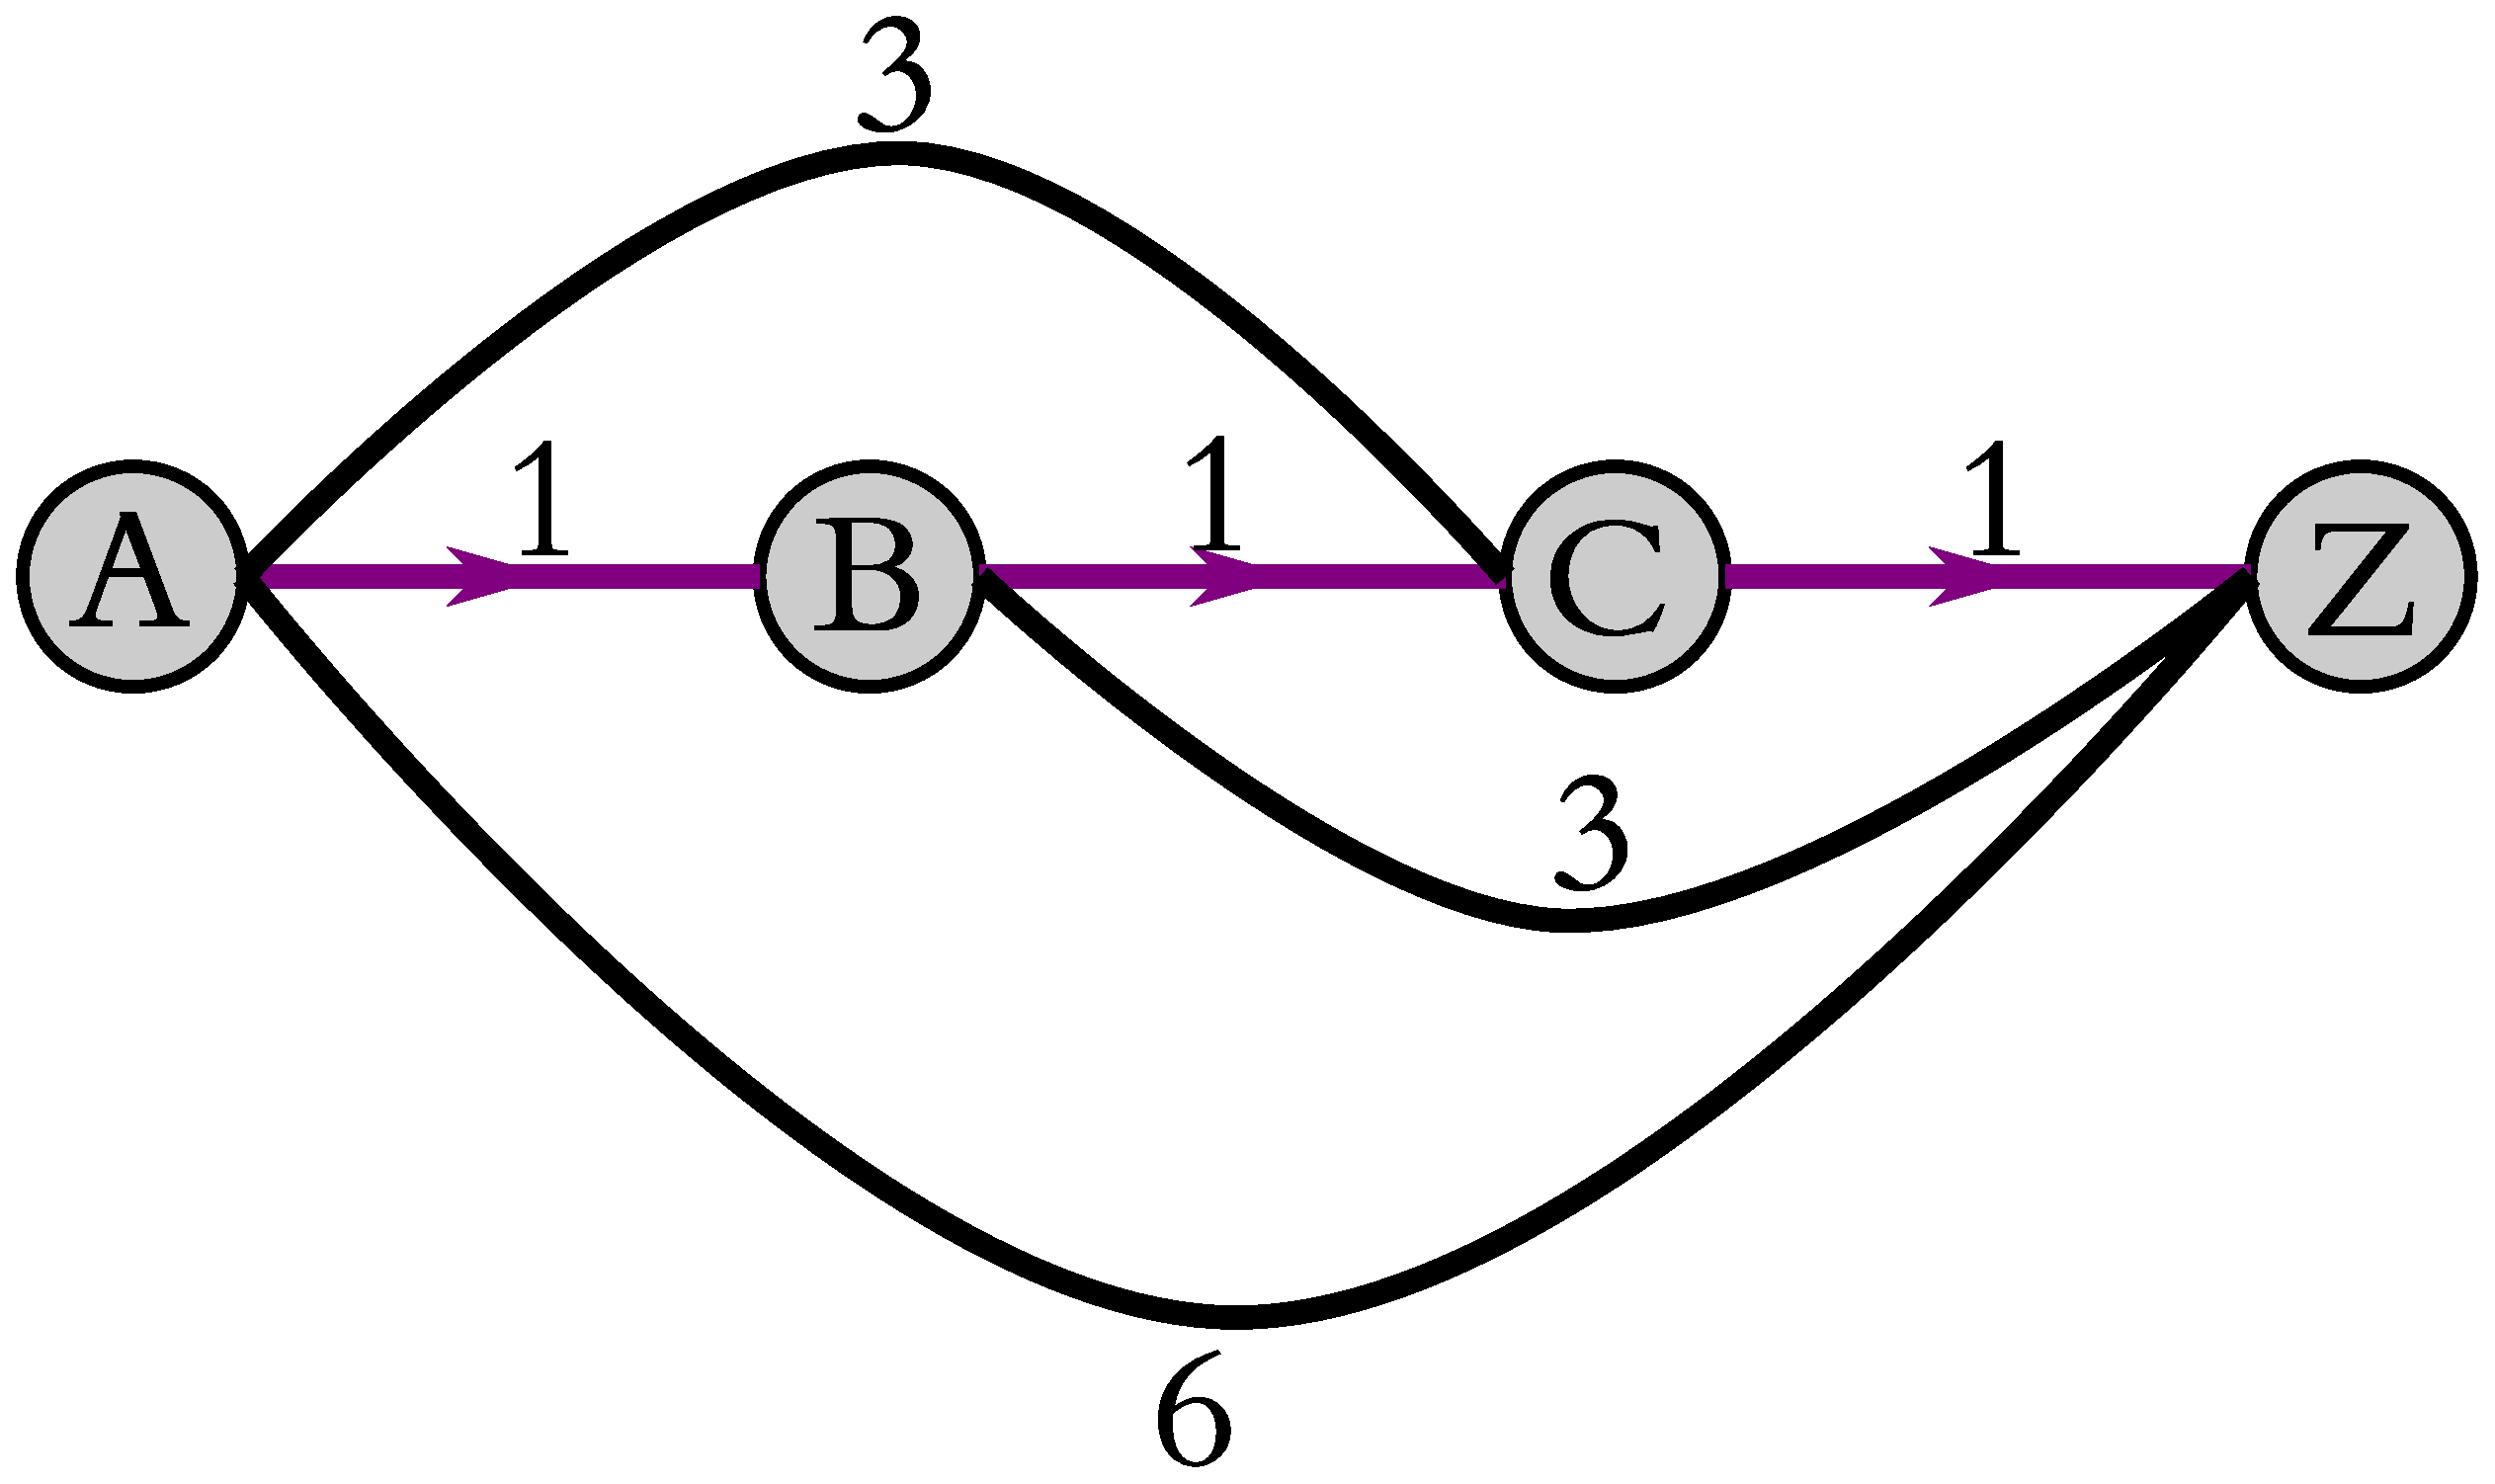
\includegraphics[width=60mm]{bhandari_suurballe1_1}
\caption{
Finding shortest path between nodes A and Z
}
\end{subfigure}
%%%%%%%%%%%%%%%%%
\begin{subfigure}{0.49\textwidth}
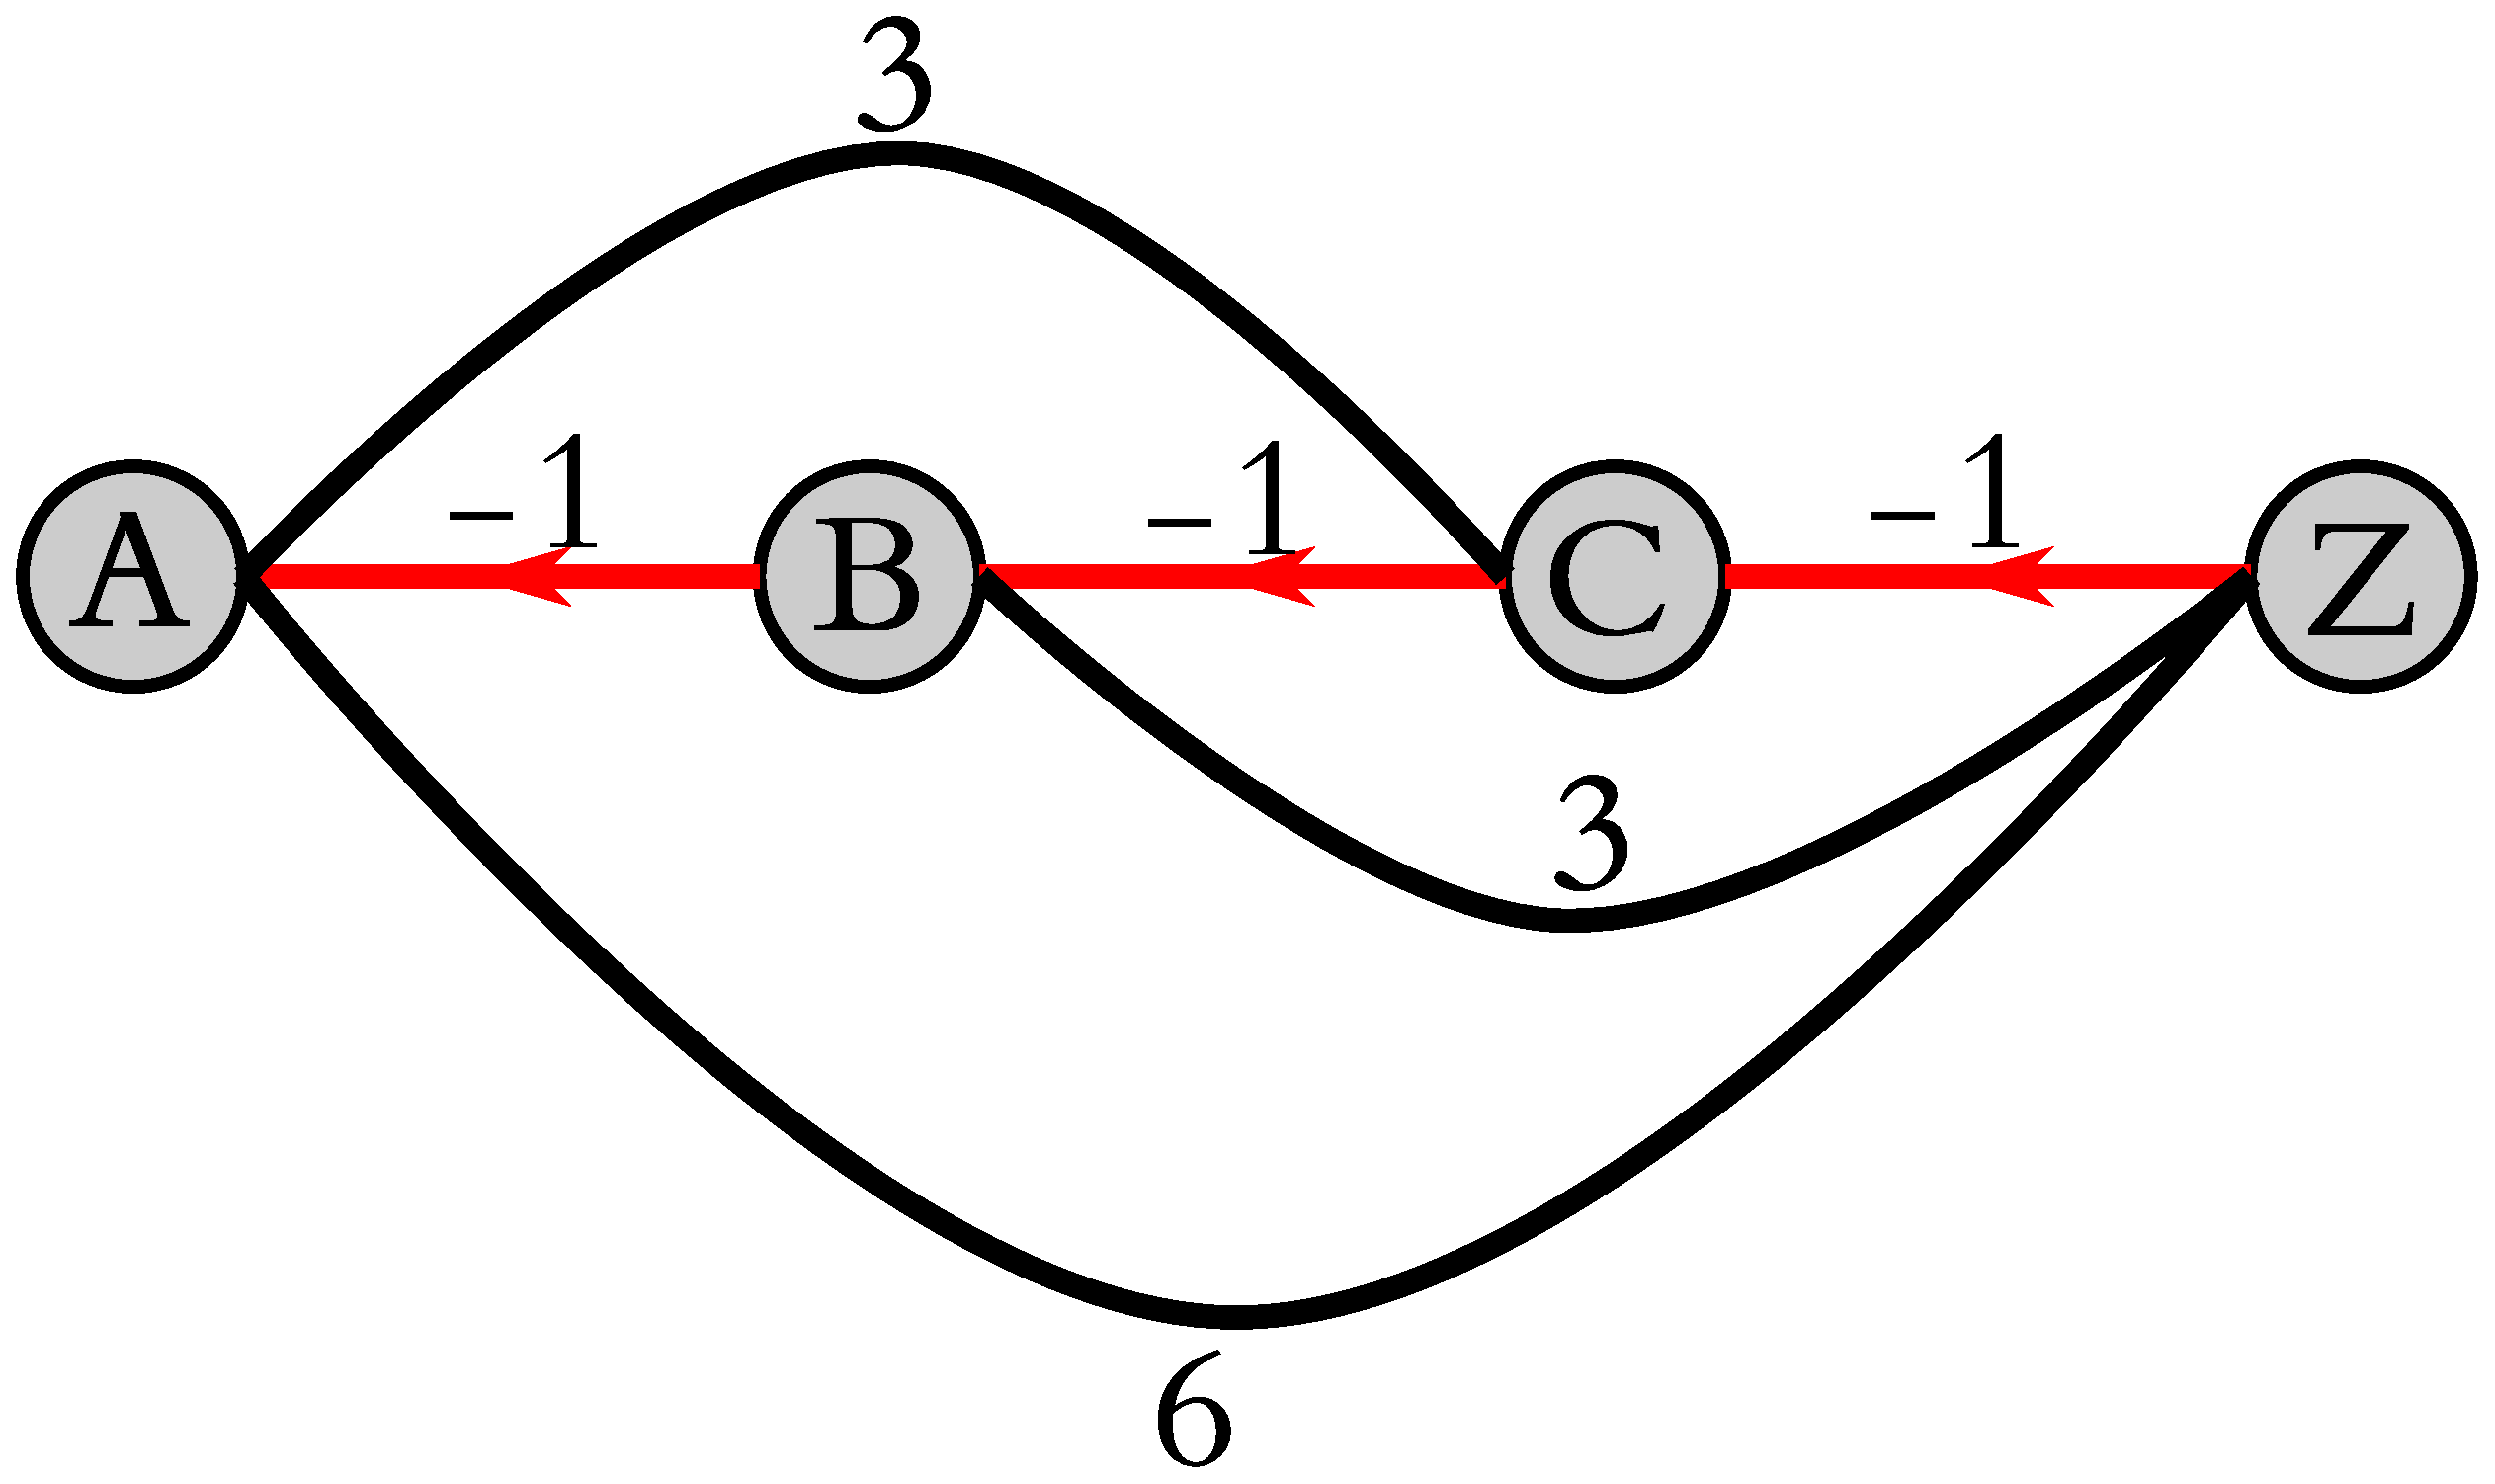
\includegraphics[width=60mm]{bhandari_suurballe1_2}
\caption{
Reversing link direction and link cost along the shortest path
}
\end{subfigure}
%%%%%%%%%%%%%%%%%
\begin{subfigure}{0.49\textwidth}
\includegraphics[width=60mm]{bhandari_suurballe1_3}
\caption{
Finding the second shortest path between nodes A and Z
}
\end{subfigure}
%%%%%%%%%%%%%%%%%
\begin{subfigure}{0.49\textwidth}
\includegraphics[width=60mm]{bhandari_suurballe1_4}
\caption{
Removing common links among the two shortest paths found
}
\end{subfigure}
%%%%%%%%%%%%%%%%%
\caption{
The steps of Bhandari algorithm
}
\label{fig:bhandari}
\end{figure}

\begin{figure}[h]
\centering
%%%%%%%%%%%%%%%%%
\begin{subfigure}{0.49\textwidth}
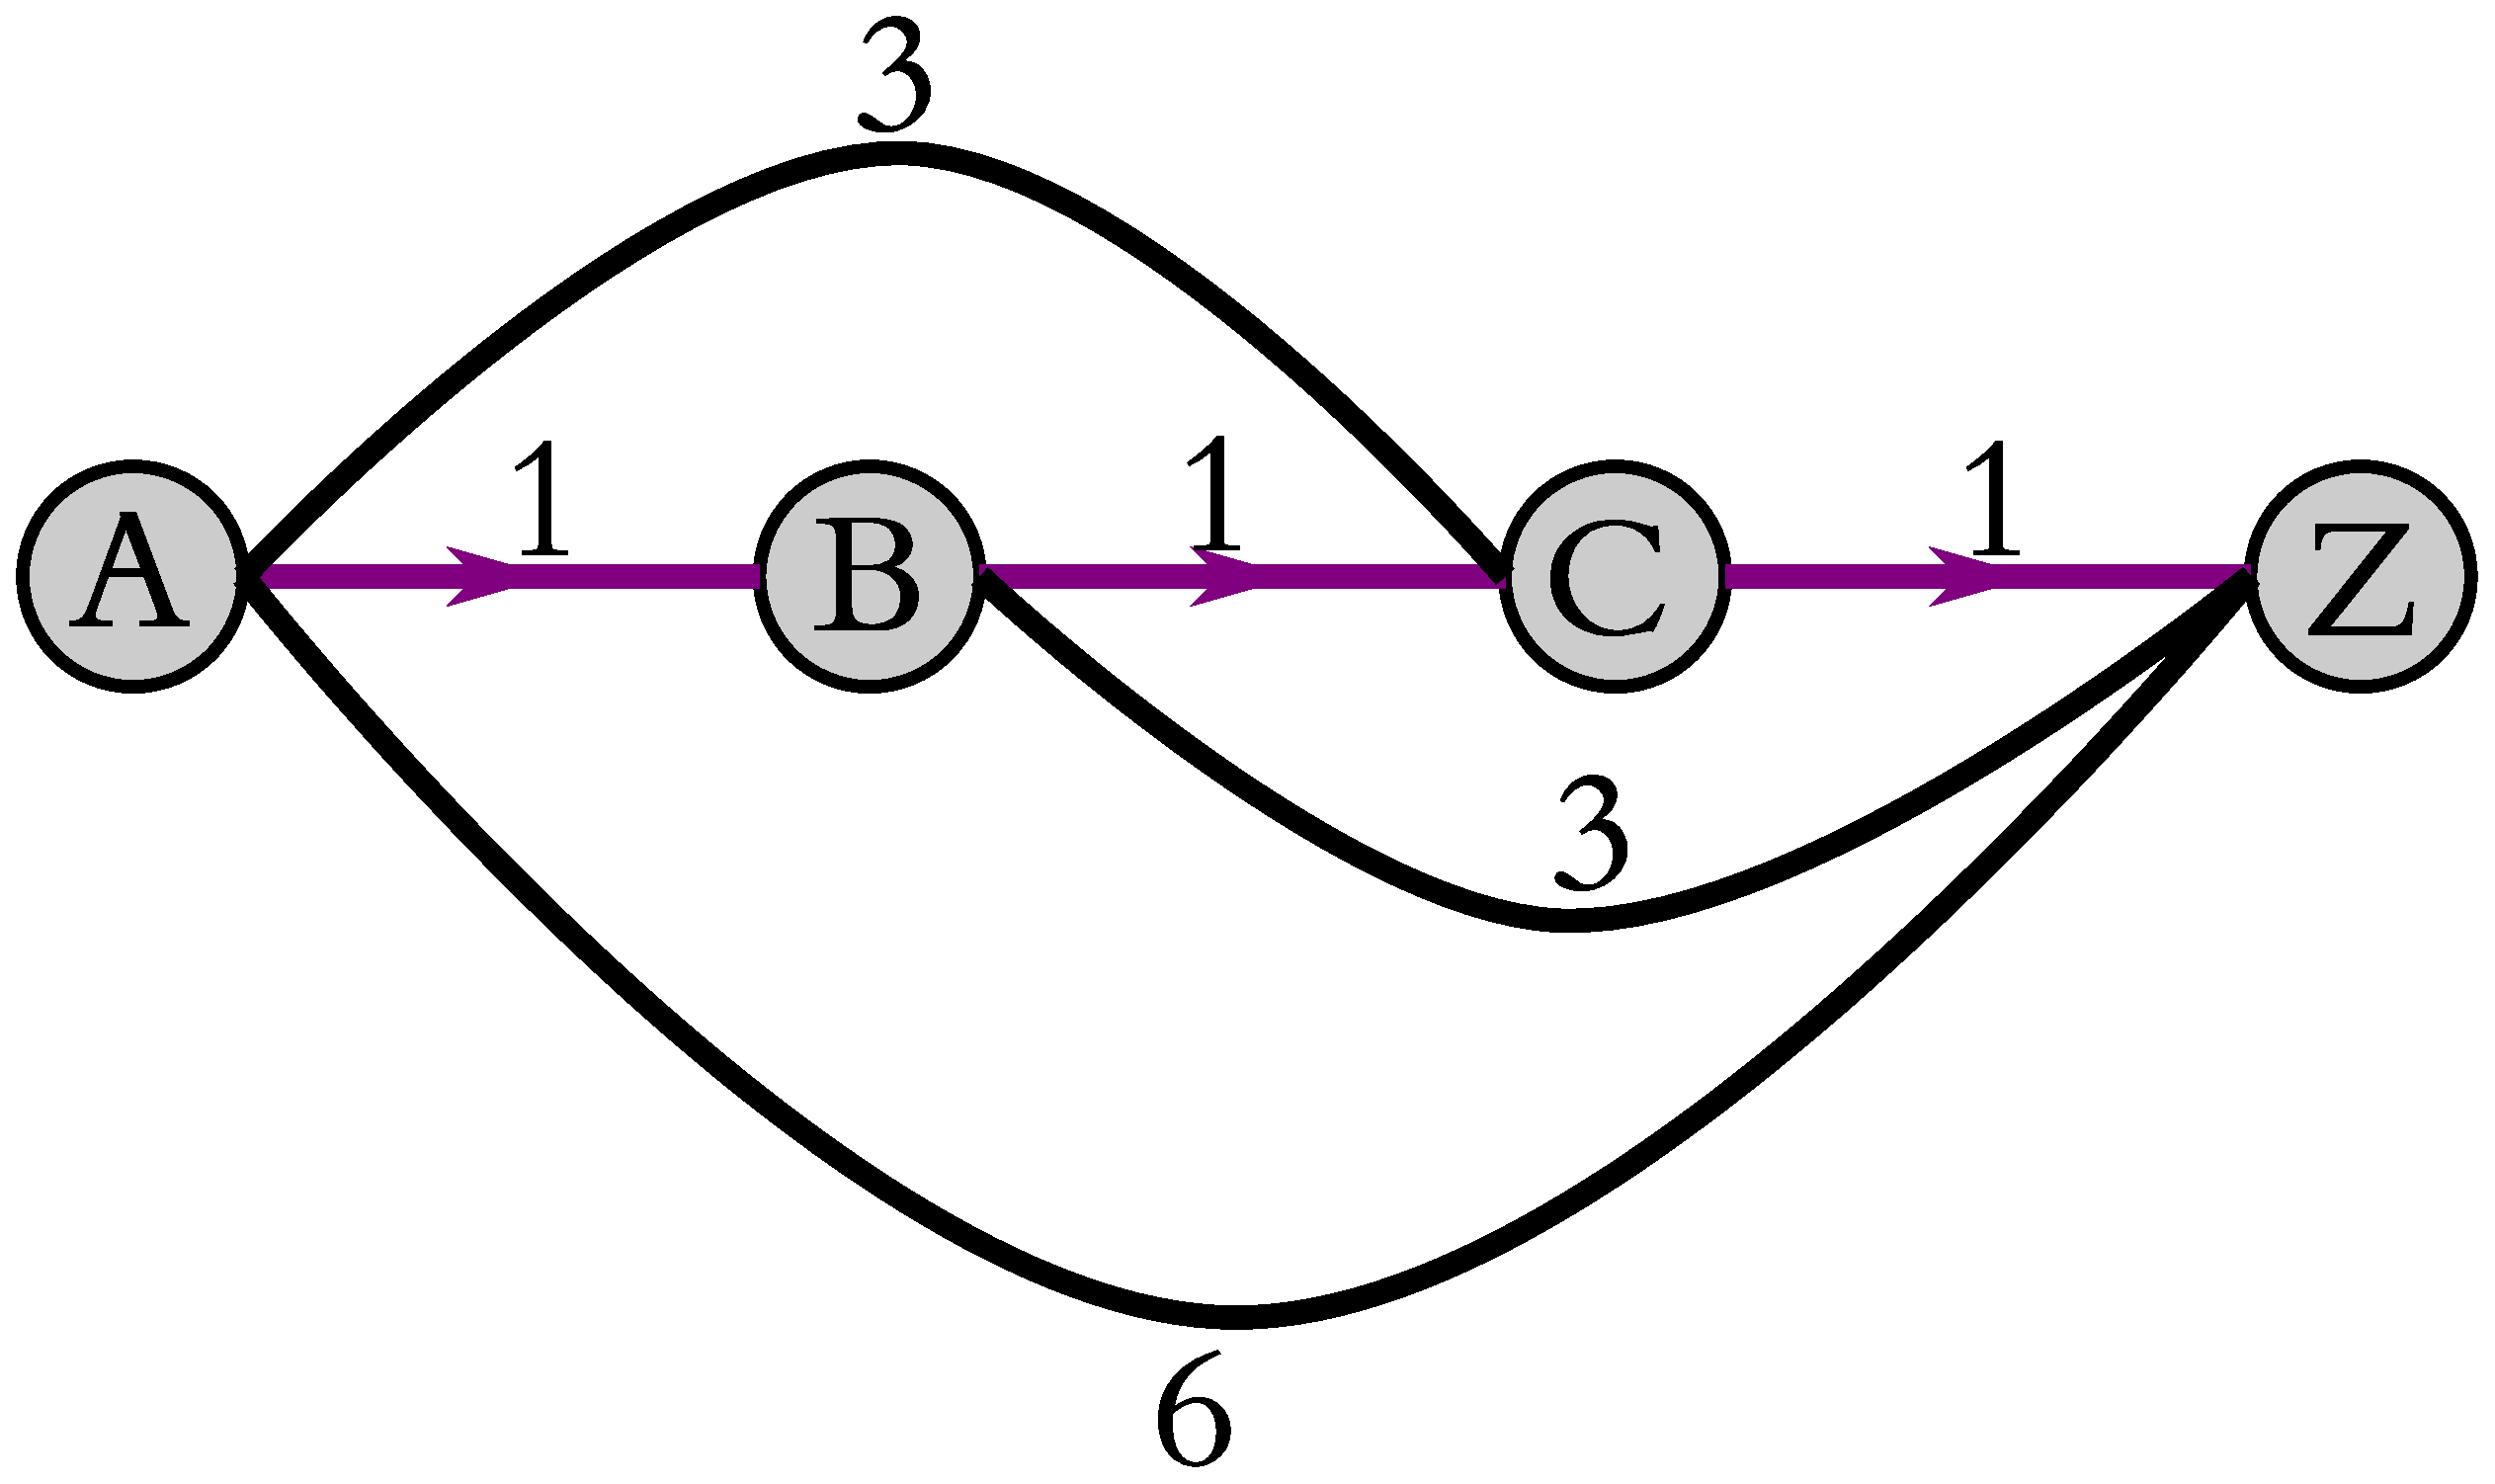
\includegraphics[width=60mm]{bhandari_suurballe1_1}
\caption{
Finding shortest paths from source node to all other nodes
}
\end{subfigure}
%%%%%%%%%%%%%%%%%
\begin{subfigure}{0.49\textwidth}
\includegraphics[width=60mm]{bhandari_suurballe2_2}
\caption{
Updating costs of all links according to 
$
w_\text{new}(u,v)
=
w_\text{old}(u,v)+d(s,u)-d(s,v)
$
and reversing link direction along the shortest path ($d(s,u)$ is the minimum cost of reaching node $u$ from $s$)
}
\end{subfigure}
%%%%%%%%%%%%%%%%%
\begin{subfigure}{0.49\textwidth}
\includegraphics[width=60mm]{bhandari_suurballe2_3}
\caption{
Reversing link direction along the shortest path tree
}
\end{subfigure}
%%%%%%%%%%%%%%%%%
\begin{subfigure}{0.49\textwidth}
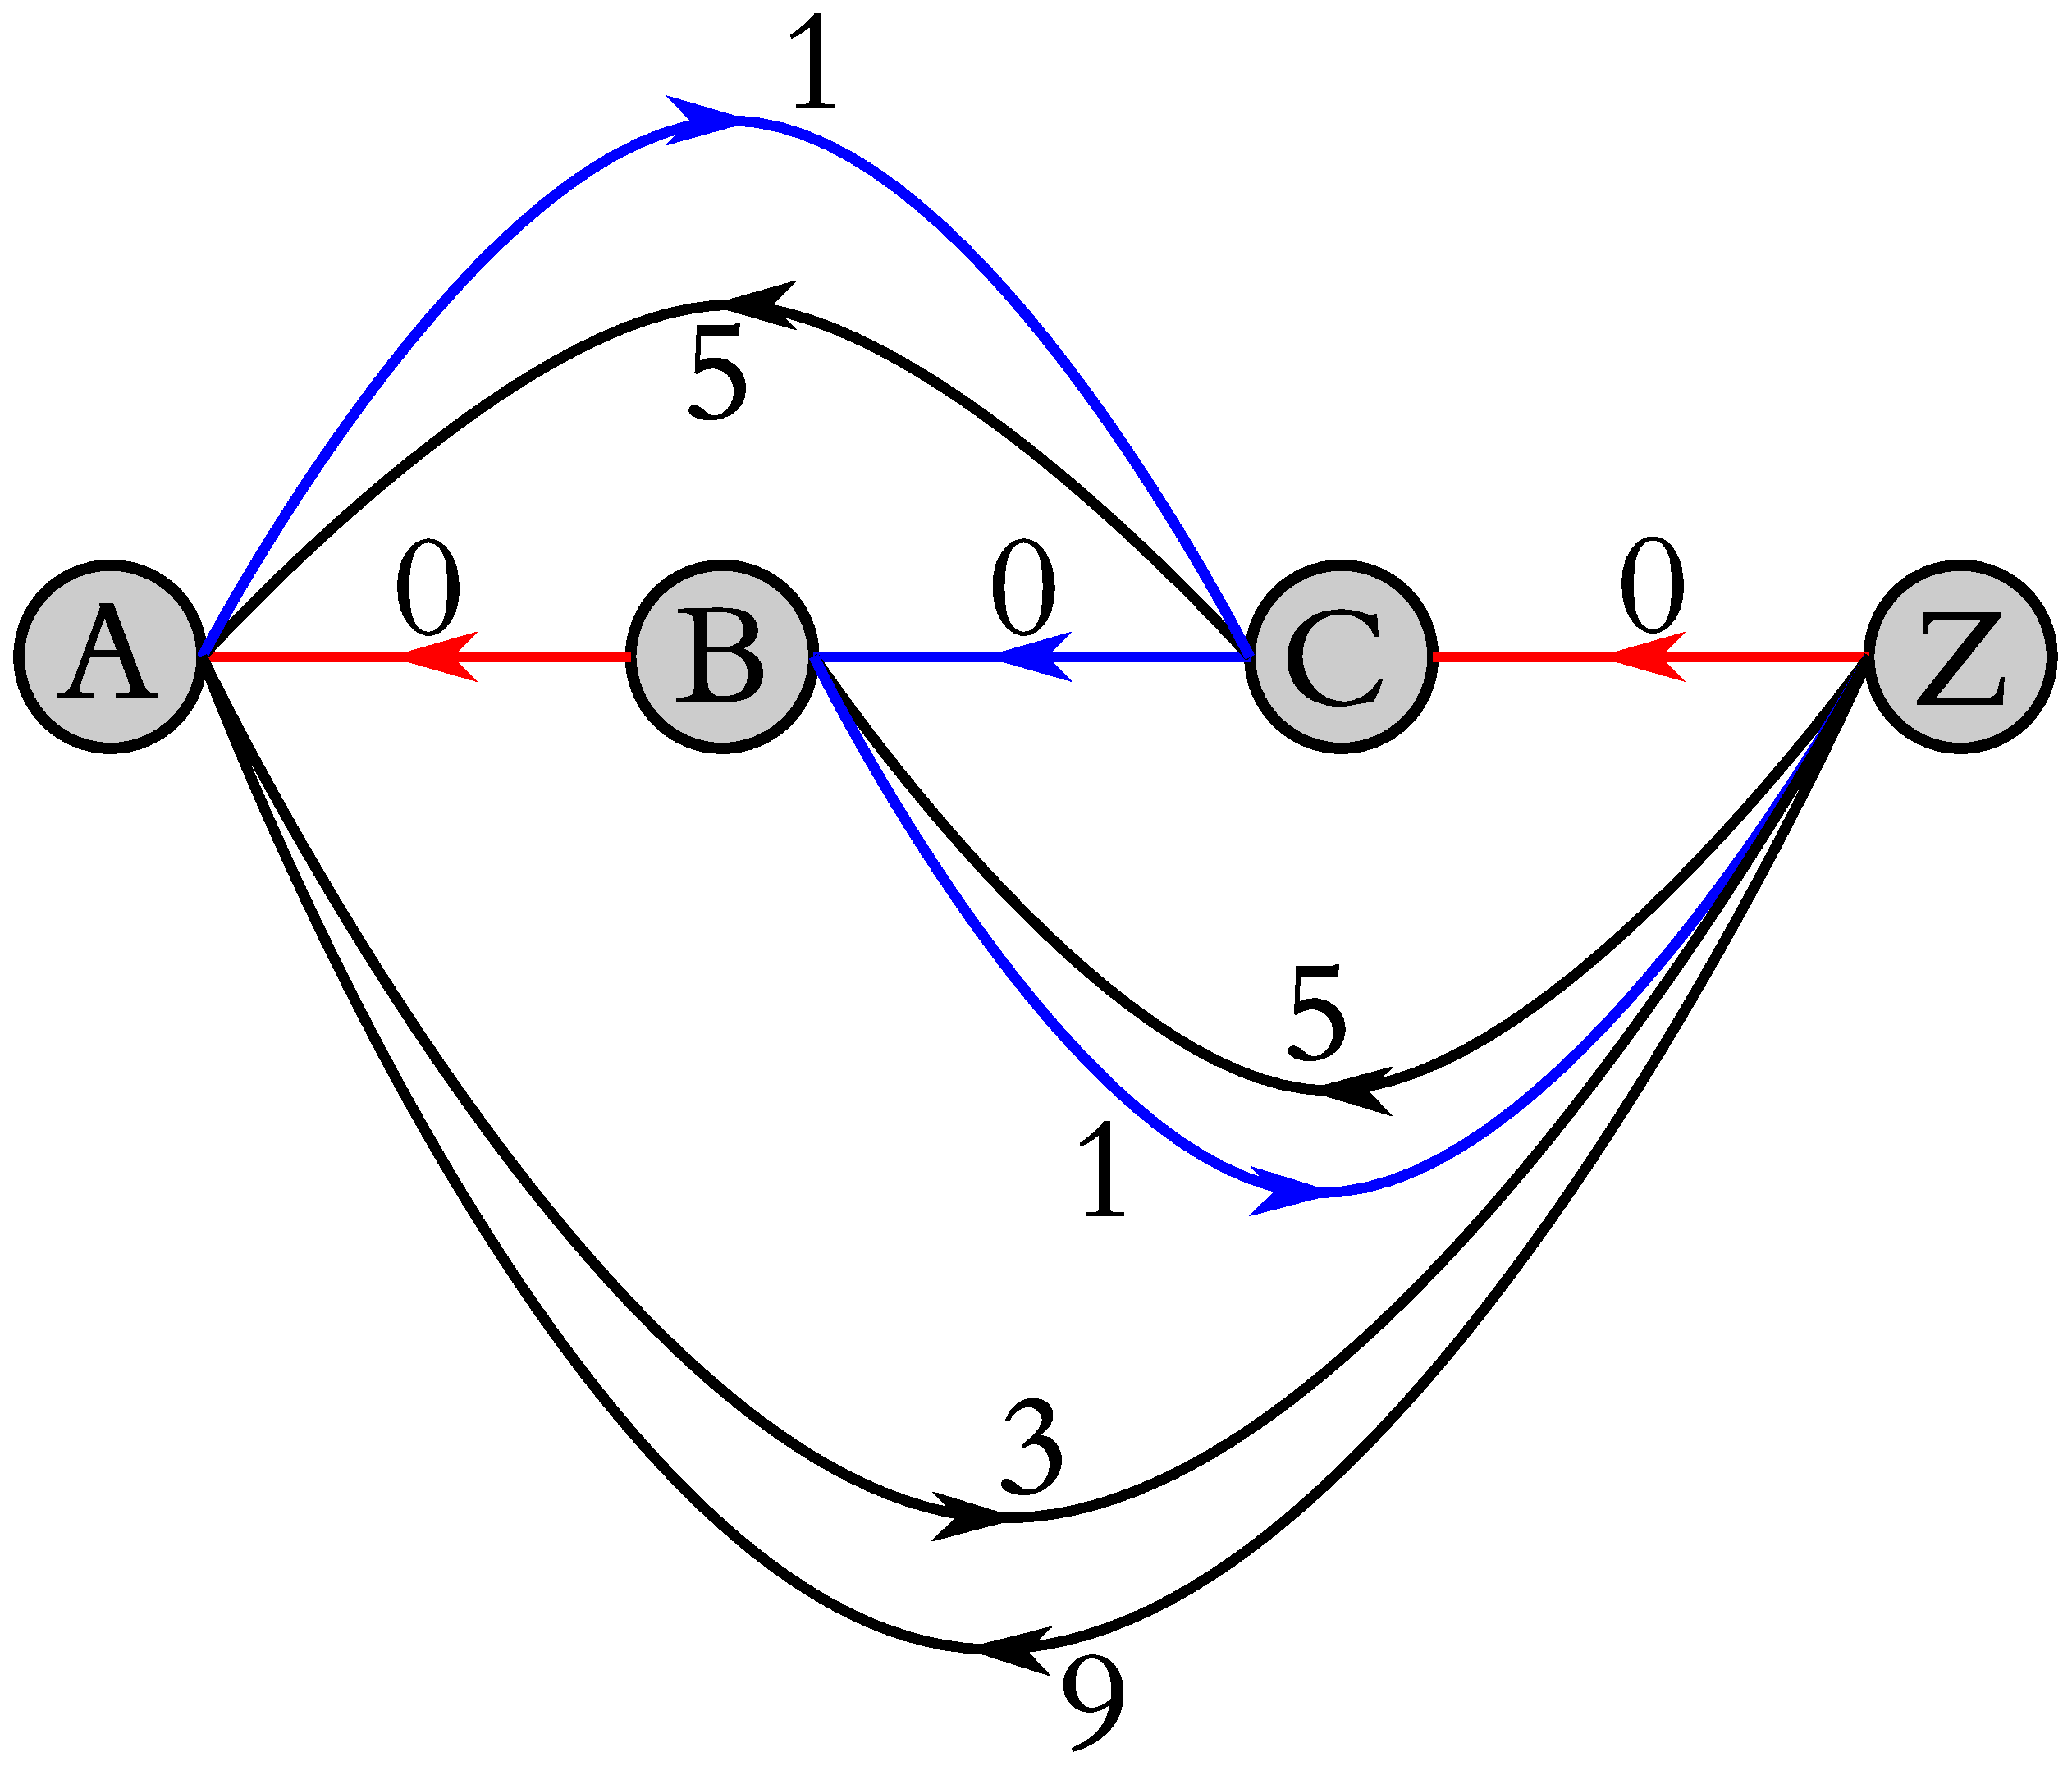
\includegraphics[width=60mm]{bhandari_suurballe2_4}
\caption{
Calculating a new shortest path between nodes A and Z
}
\end{subfigure}
%%%%%%%%%%%%%%%%%
\begin{subfigure}{0.49\textwidth}
\includegraphics[width=60mm]{bhandari_suurballe1_4}
\caption{
Removing common links among the two shortest paths found
}
\end{subfigure}
%%%%%%%%%%%%%%%%%
\caption{
The steps of Suurballe's algorithm
}
\label{fig:suurballe}
\end{figure}

\Q

The NF of Raman amplifier as of its gain is a linear equation as follows
$$
NF_\text{Raman}(\text{dB})=aG_\text{Raman}(\text{dB})+b,
$$
where $a=-0.25$ and $b=24.25$. The total noise figure (in linear scale) is then given by the following equation
$$
NF_\text{total}=10^{-0.025G_\text{Raman}+2.425}+\frac{10^{0.6}-1}{10^{0.1G_\text{Raman}}}.
$$
Both the terms $10^{-0.025G_\text{Raman}+2.425}$ and $\frac{10^{0.6}-1}{10^{0.1G_\text{Raman}}}$ are strictly decreasing with respect to $G_\text{Raman}$, meaning that the NF reaches it minimum when $G_\text{Raman}$ reaches its maximum which is 18dB. Since the amplifiers must fully compensate the 20dB fiber loss, the EDFA gain equals 2dB. The optimum noise figure is
$$
NF_\text{opt}\approx 19.75\text{dB}.
$$

\newpage

\Q

\begin{enumerate}[label=\alph*-]
\item b-

These steps are sketched in figure \ref{fig:steiner}.

c- d- e-

Since no new nodes are added to the network, the result of step (b) is the final result.
\end{enumerate}

\begin{figure}[htbp]
\centering
\begin{subfigure}{0.49\textwidth}
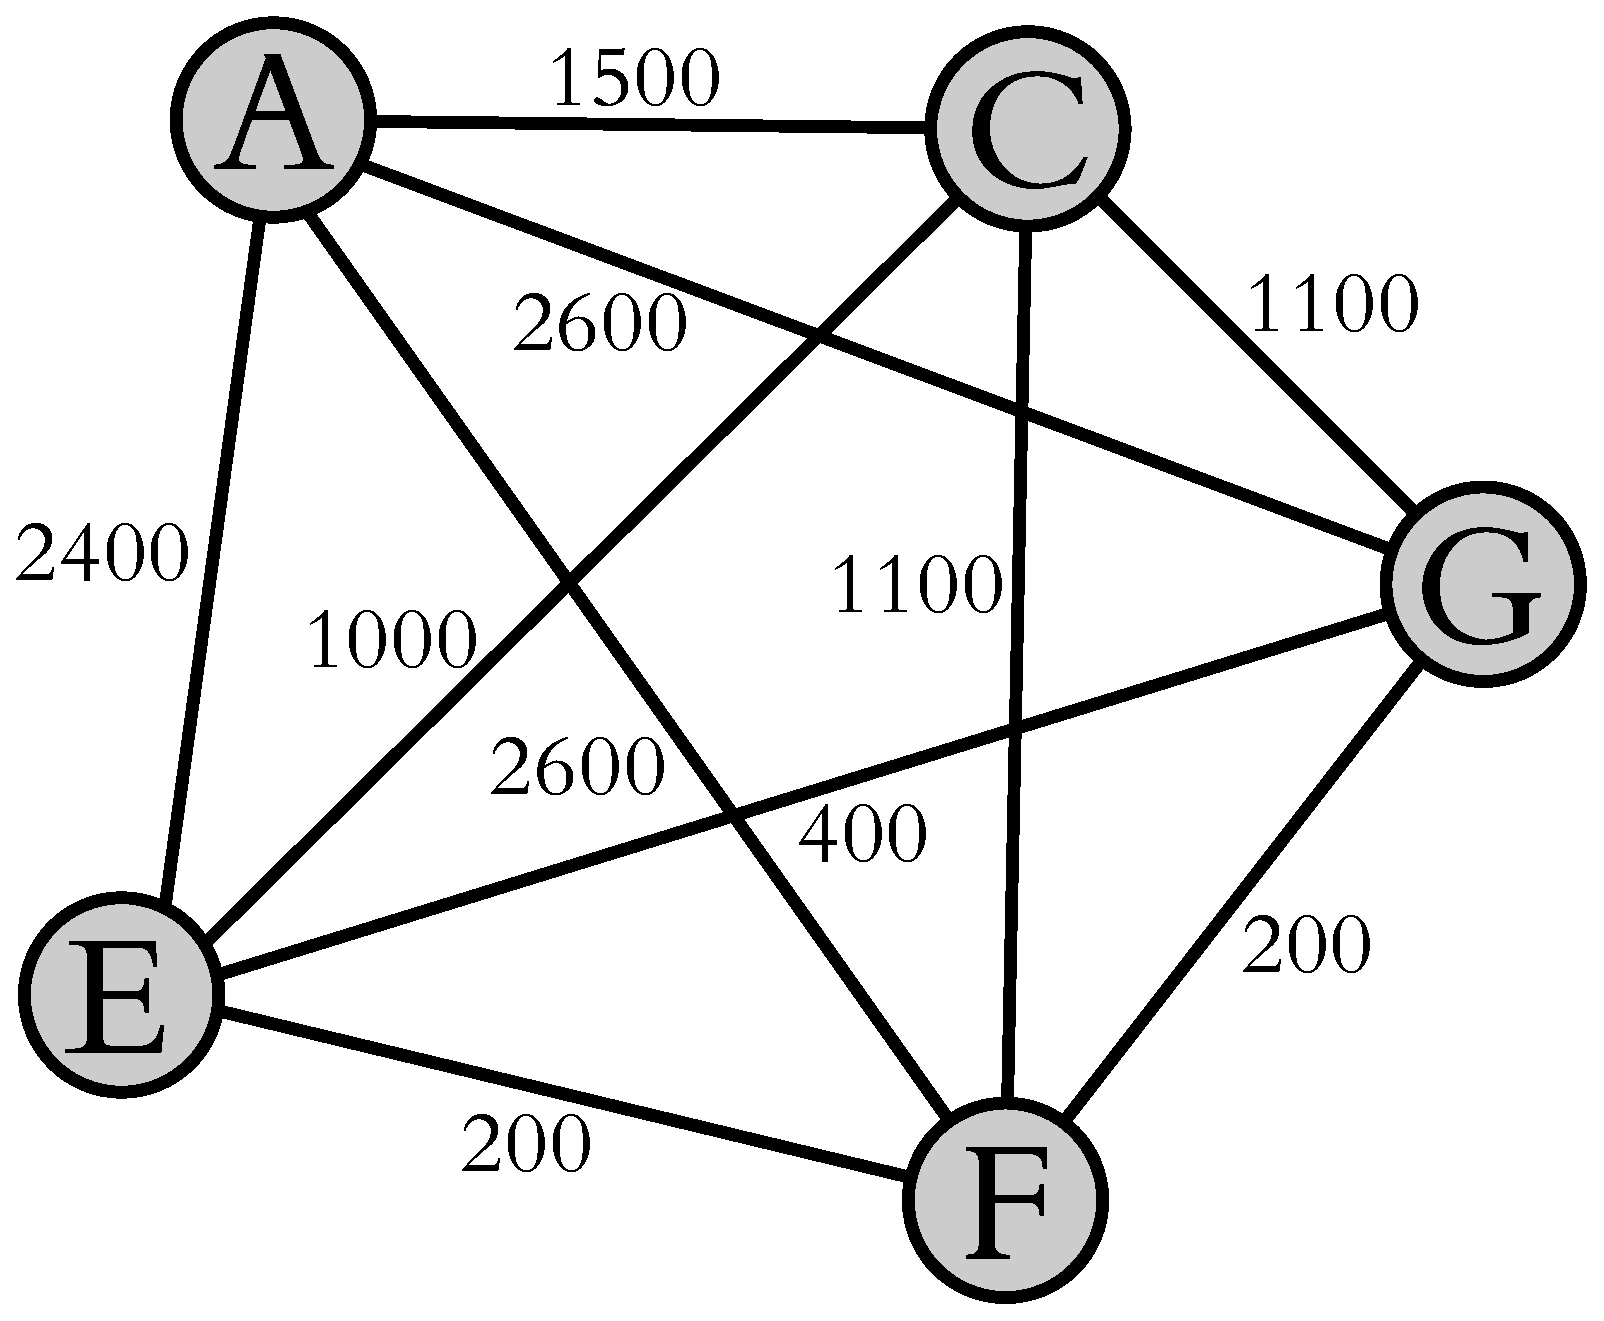
\includegraphics[width=60mm]{steiner_1}
\end{subfigure}
\begin{subfigure}{0.49\textwidth}
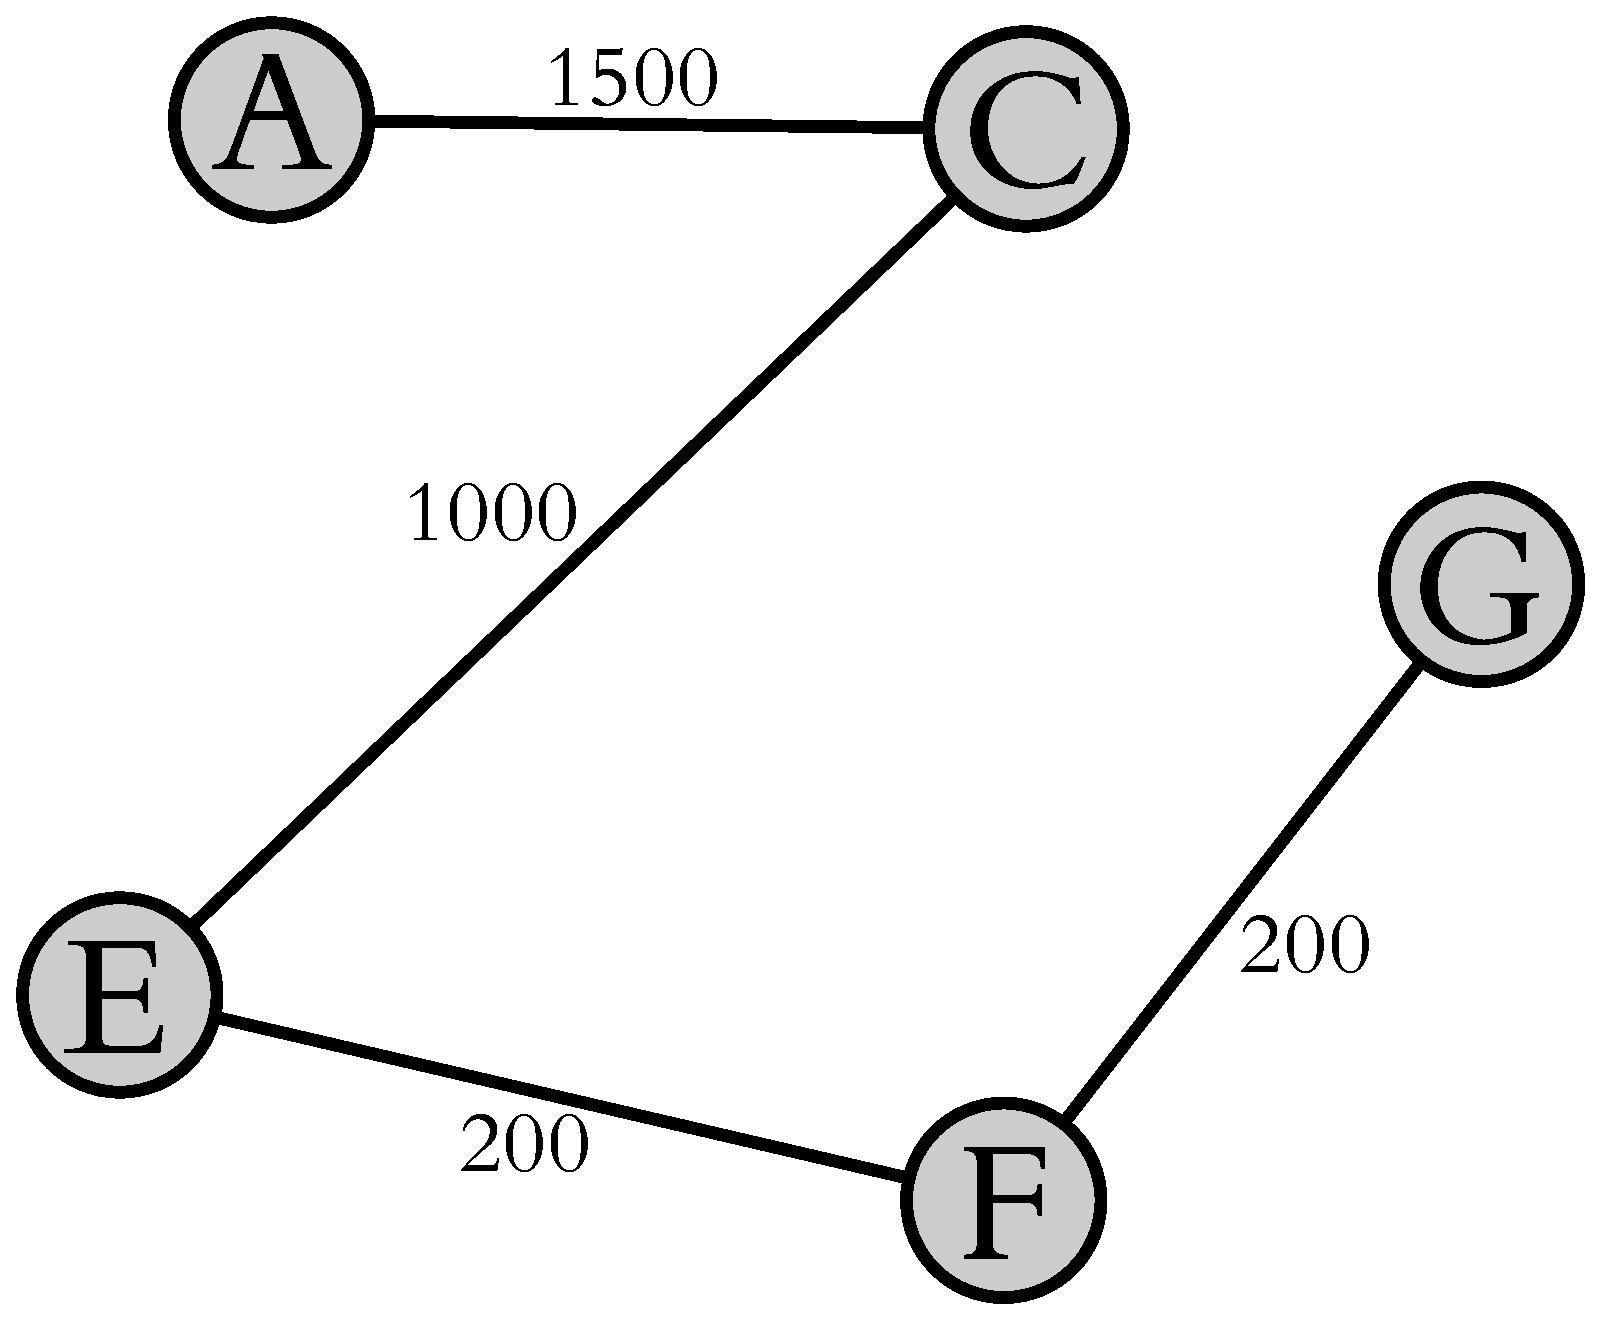
\includegraphics[width=60mm]{steiner_2}
\end{subfigure}
\caption{
The steps of MSTE hueristic
}
\label{fig:steiner}
\end{figure}
\end{document}